\chapter{Representative Model-to-Model-Transformation Scenarios}\label{chapM2MScenarios}

In order to create an automatic \gls{TransformationGenerator}, it is necessary to define representative test scenarios. Each scenario consists of two \glspl{MetaModel} and at least two semantically identical example \glspl{Model} of those (see chapter \ref{chapFoundations}). 

Designing software systems usually involves the analysis of structure and behavior, hence those categories have been chosen for the scenarios (see chapter \ref{chapIntroduction}), to show the relevance of the transformations. However, in terms of the transformation complexity the category does not matter.

The starting point is a simple structural scenario, while the complex one is a behavioral scenario.

\section{Simple Structural Scenario}\label{secM2MScenarioStructuralSimple}

As a result of the analysis in section \ref{secTransformationComplexity}, the simple structural example requires only a 1:1 transformation of \glspl{MetaObjectFacility} \glspl{Class}, \glspl{Association} and ``Name"-\glspl{Property}.

\begin{figure}[htb]
	\centering
	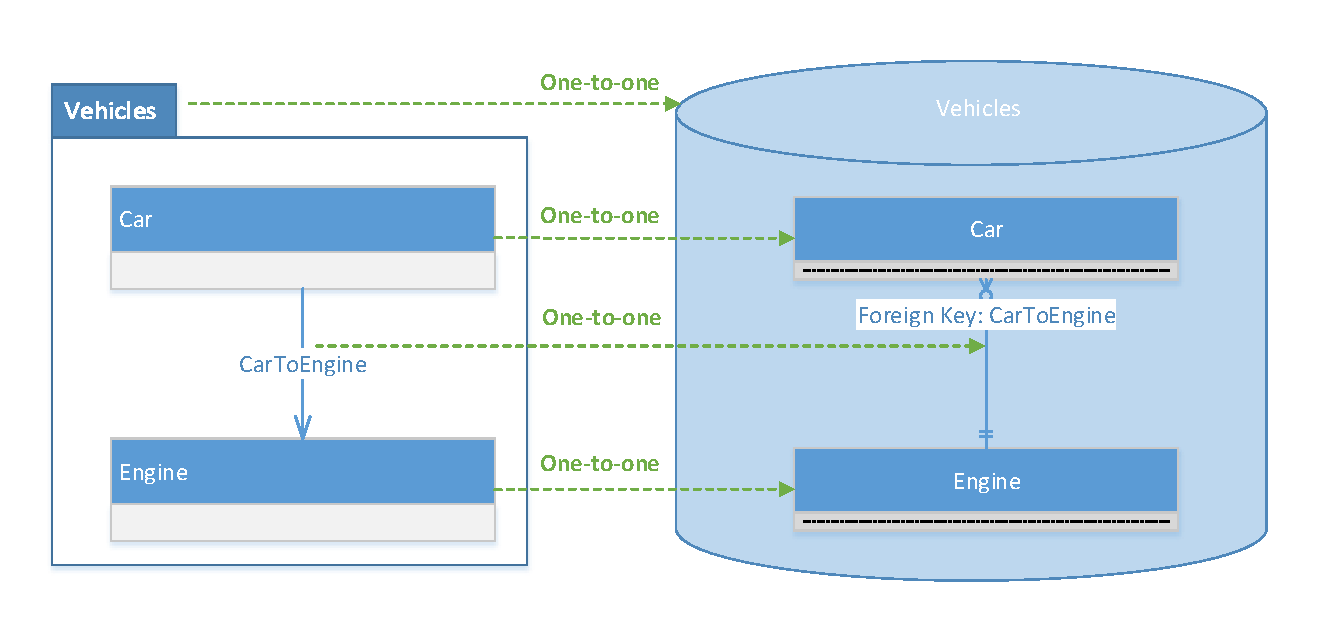
\includegraphics[scale=0.6, trim=0cm 1cm 0cm 1cm, clip=true]{Images/ScenarioStructuralSimpleOverview.pdf} 
	\caption{Simple transformation scenario overview with a \Gls{UnifiedModelingLanguage} \gls{ClassDiagram} \gls{Model} on the left side and an equivalent \gls{RelationalSchema} \gls{Model} on the right side, both in \gls{ConcreteSyntax}}
	\label{figScenarioStructuralSimpleOverview}
\end{figure}

A common scenario in the field of \gls{ModelDrivenDevelopment} is the already mentioned transformation of a \gls{UnifiedModelingLanguage} \gls{ClassDiagram} to a \gls{RelationalSchema}. Figure \ref{figScenarioStructuralSimpleOverview} shows the transformation scenario based on an example. In order to have 1:1 transformations on the \gls{MetaModel} and \gls{Model} level, only the core concepts are used. The \gls{ClassDiagram} consists of a package ``Vehicles", the \glspl{Class} ``Car" and ``Engine", as well as an \gls{Association} between those. The \gls{RelationalSchema} has a database schema ``Vehicles", the tables ``Car" and ``Engine", and a foreign-key in table ``Car" which points to the table ``Engine".

In the following paragraphs the \glspl{MetaModel}, the \gls{ModelToModelTransformation} and the example \glspl{Model} are presented.

It has to be pointed out that the terms \gls{Class} and \gls{Property} exist in both, the \glspl{MetaObjectFacility} and the \gls{ClassDiagram}.

The reduced \gls{UnifiedModelingLanguage} \gls{ClassDiagram} \gls{MetaModel} shown in figure \ref{figScenarioStructuralSimpleUmlClassMetaModel} consists of a ``UmlPackage" that contains ``UmlClasses" and ``UmlAssociations". The former may be associated by the latter to another ``UmlClass". Therefore, a ``UmlAssociation" has a ``Source" and ``Target" association.

\begin{figure}[htb]
	\centering
	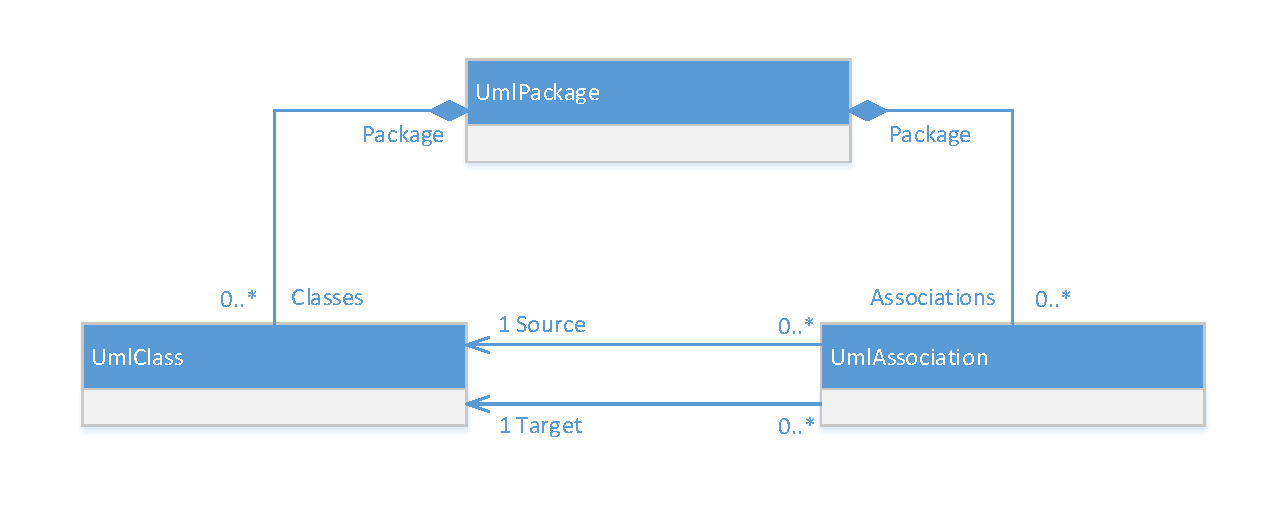
\includegraphics[scale=0.6, trim=0cm 1cm 0cm 1cm, clip=true]{Images/ScenarioStructuralSimpleUmlClassMetaModel.pdf} 
	\caption{\Gls{UnifiedModelingLanguage} \gls{ClassDiagram} - simplified \gls{MetaModel}}
	\label{figScenarioStructuralSimpleUmlClassMetaModel}
\end{figure}

The simplified \gls{RelationalSchema} \gls{MetaModel} is shown in figure \ref{figScenarioStructuralSimpleRelationalMetaModel}. It includes a ``RelationalSchema" that contains ``RelationalTables". The latter may refer to others of the same kind via a ``RelationalForeignKey" that has an association named ``ReferencedTable". The difference to the \gls{UnifiedModelingLanguage} \gls{ClassDiagram} \gls{MetaModel} is that the ``ForeignKey" is only associated to the owning ``Table" and not to the ``RelationalSchema". Hence, this association has no equivalence and requires no mapping.

\begin{figure}[htb]
	\centering
	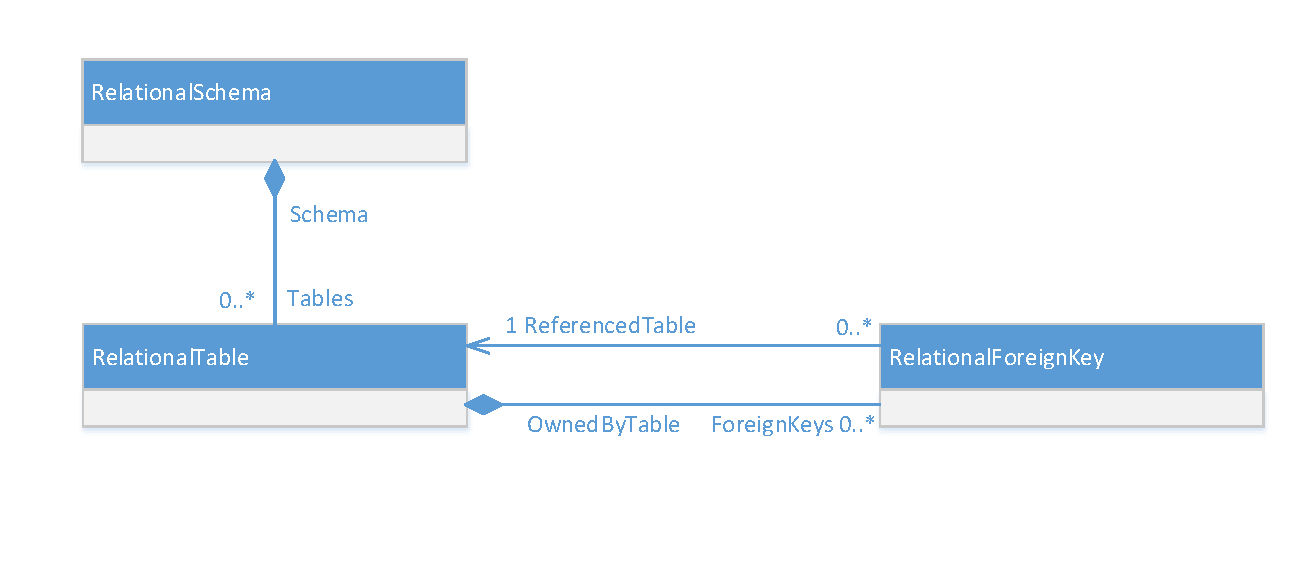
\includegraphics[scale=0.6, trim=0cm 1cm 0cm 1cm, clip=true]{Images/ScenarioStructuralSimpleRelationalMetaModel.pdf} 
	\caption{\Gls{RelationalSchema} - simplified \gls{MetaModel}}
	\label{figScenarioStructuralSimpleRelationalMetaModel}
\end{figure}

A transformation that converts the first \gls{MetaModel} into the second one is presented in listing \ref{lstETLSimpleExample}. This is a valid transformation, but it is not the only one, since there are other possible solutions. The presented one contains three rules, one for each \gls{MetaObjectFacility} \gls{Class}, resulting in the \glspl{TransformationRule} ``UmlPackage To RelationalSchema", ``UmlClass To RelationalTable", ``UmlAssociation To RelationalForeignKey". All rules have a mapping for the ``Name" \gls{Property}. Additionally, ``UmlClass To RelationalTable" maps the associated ``UmlPackage" of the ``UmlClass" to the corresponding ``RelationalSchema" of the created ``RelationalTable" with the keyword ``equivalent". The rule ``UmlAssociation To RelationalForeignKey" contains mappings for the ``Source" and ``Target" to the corresponding \glspl{Property} of the \gls{RelationalSchema}.

\begin{lstlisting}[language=ETL,caption={Simple \gls{UnifiedModelingLanguage} \gls{ClassDiagram} to simple \gls{RelationalSchema} \gls{ModelToModelTransformation} in \gls{ConcreteSyntax} of \gls{EpsilonTransformationLanguage}},label={lstETLSimpleExample}]
rule UmlPackageToRelationalSchema
  	transform umlPackage : Source!UmlPackage
  	to relationalSchema : Target!RelationalSchema {
  
  	relationalSchema.Name = umlPackage.Name; 
}

rule UmlClassToRelationalTable 
	transform umlClass : Source!UmlClass
	to relationalTable : Target!RelationalTable {
	
	relationalTable.Name = umlClass.Name;
	relationalTable.Schema = umlClass.Package.equivalent();
}

rule UmlAssociationToRelationalForeignKey
	transform umlAssociation : Source!UmlAssociation
	to relationalForeignKey : Target!RelationalForeignKey {
	
	relationalForeignKey.Name = umlAssociation.Name;
	relationalForeignKey.OwnedByTable = umlAssociation.Source.equivalent();
	relationalForeignKey.ReferencedTable = umlAssociation.Target.equivalent();	
}
\end{lstlisting}

In order to identify a transformation with the \gls{TransformationGenerator} also at least one example \gls{Model} pair for those two \glspl{MetaModel} has to be defined. It is required for them to be semantically equivalent. Figure \ref{figScenarioStructuralSimpleUmlClassModel1} shows a \gls{Model} conforming to the \Gls{UnifiedModelingLanguage} \gls{ClassDiagram} \gls{MetaModel}. It contains a ``UmlPackage" named ``Vehicles" that defines the context. Inside this package are a ``Car" and an ``Engine" which are ``UmlClasses". Those are associated by a ``Car 2 Engine" ``UmlAssociation". 

\begin{figure}[htb]
	\centering
	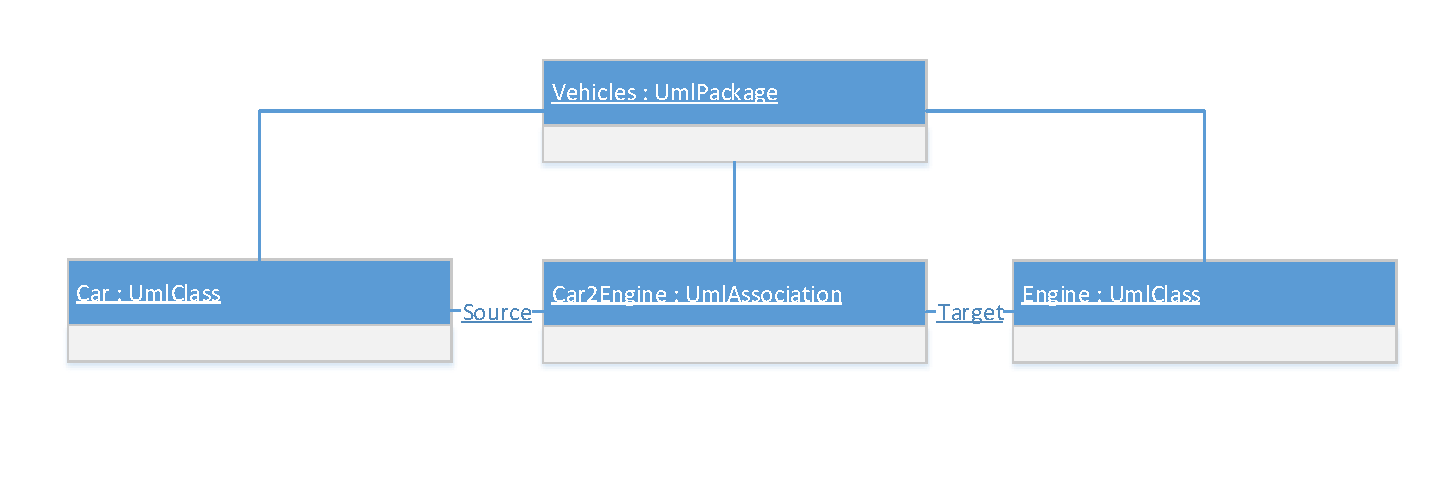
\includegraphics[scale=0.6, trim=0cm 1cm 0cm 1cm, clip=true]{Images/ScenarioStructuralSimpleUmlClassModel1.pdf} 
	\caption{\Gls{UnifiedModelingLanguage} \gls{ClassDiagram} example \gls{Model}}
	\label{figScenarioStructuralSimpleUmlClassModel1}
\end{figure}

The semantically identical \gls{Model}, conforming to the \gls{RelationalSchema} \gls{MetaModel}, is presented in figure \ref{figScenarioStructuralSimpleRelationalModel1}.

%It has to be pointed out that the containment relationship between the ``RelationalTable" ``Car" and the ``Car 2 Engine" ``RelationalForeignkey" is only visible in the presentation of the \gls{MetaModel}.

\begin{figure}[htb]
	\centering
	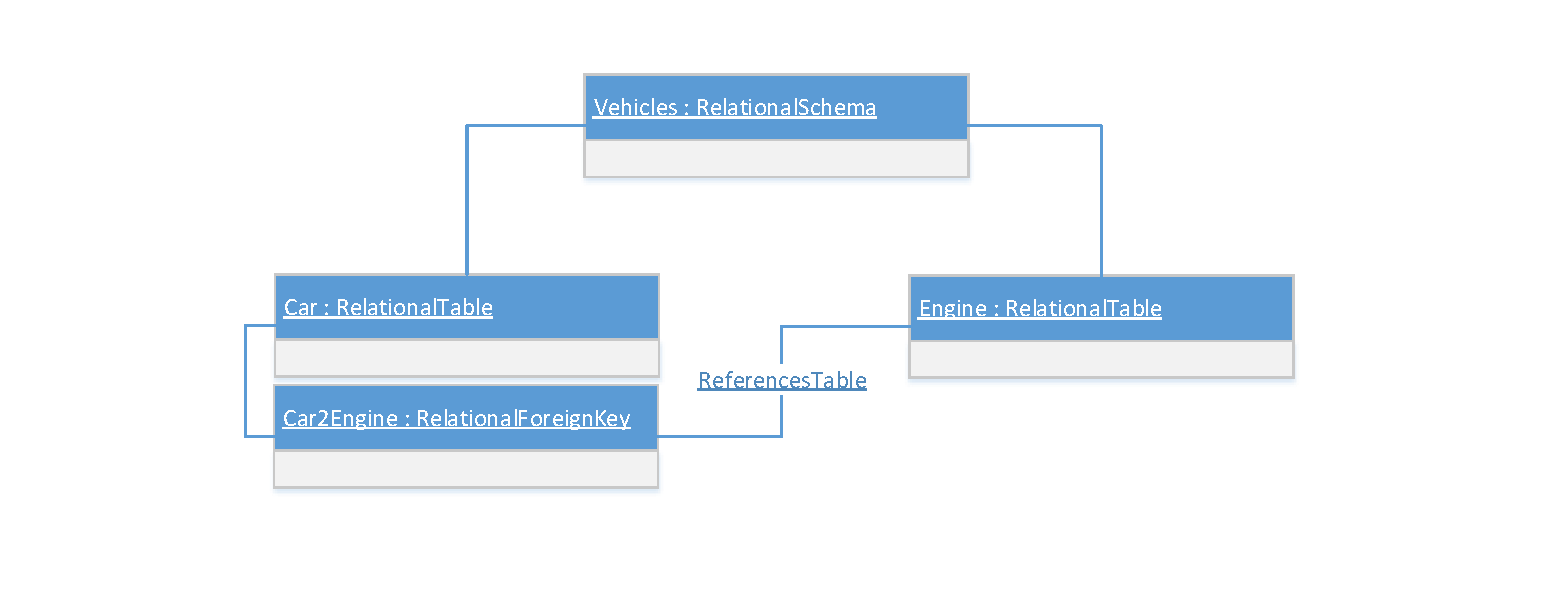
\includegraphics[scale=0.6, trim=0cm 1cm 0cm 1cm, clip=true]{Images/ScenarioStructuralSimpleRelationalModel1.pdf} 
	\caption{\Gls{RelationalSchema} example \gls{Model}}
	\label{figScenarioStructuralSimpleRelationalModel1}
\end{figure}

\section{Complex Behavioral Scenario}\label{secM2MScenarioBehavioralComplex}

According to the identified complexity levels in section \ref{secTransformationComplexity}, the complex example contains 1:N relations, relations that exist only under certain conditions and attribute calculations on M1.

The scenario is also common in the field of \gls{SoftwareEngineering}, which is necessary in order to show the relevance of the transformation. Compiler design is based on the concept of finite-\glspl{StateMachine}, which basically defines states and transitions between those. Since this is a low-level concept, the instances can become very large and hence difficult to read for humans. The concept of hierarchical-\glspl{StateMachine} has been introduced, which adds composite states that contain states. Thereby, the number of explicit transitions is reduced. Nevertheless, hierarchical-\glspl{StateMachine}, called complex-\glspl{StateMachine} in the following, cannot always be executed and therefore must be transformed back into (flat)-\glspl{StateMachine}, called simple-\glspl{StateMachine} in the following.

\begin{figure}[htb]
	\centering
	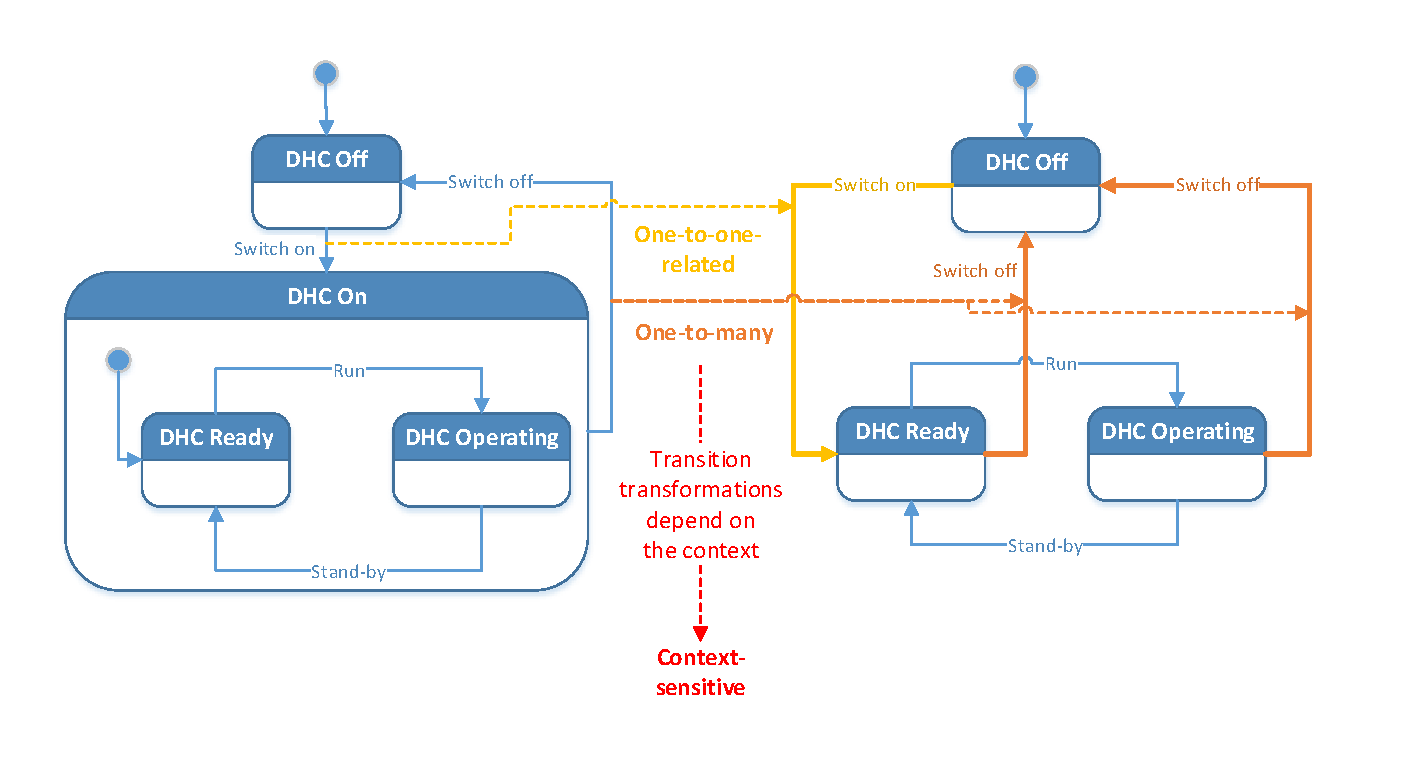
\includegraphics[scale=0.6, trim=0cm 1cm 0cm 1cm, clip=true]{Images/ScenarioBehavioralStateMachineTransformationOverview.pdf} 
	\caption{Complex transformation scenario overview with \glspl{StateMachine} in \gls{ConcreteSyntax}}
	\label{figScenarioBehavioralStateMachineTransformationOverview}
\end{figure}

Figure \ref{figScenarioBehavioralStateMachineTransformationOverview} shows an example of such a transformation and highlights the additional transformation challenges. The ``DHC" example is derived from \cite{Gerth2014} which is based on \cite{Engels2004} and models a warehouse management system. In the reduced example the ``DHC" only has the state ``DHC Off" and the complex state ``DHC On". Within the latter the machine starts in the state ``DHC Ready" and can switch to ``DHC Operating" and back. Since the complex state contains a transition to ``DHC Off", the machine can be turned off in every state inside.

The simple \gls{StateMachine} on the right hand side does not have the complex state. Therefore, the transition from ``DHC Off" to ``DHC On" points instead directly to ``DHC Ready". This results in a 1:1 transformation on M2 and M1, but the target of the transition is not the equivalent \gls{Class}, which does not exist anymore. Rather, the target is the initial state within in the composite state, therefore this is called ``One-to-one related". The outgoing transition from ``DHC On" to ``DHC Off" has to be replaced by a transition from every state inside the composite state which is called ``One-to-many". Since there are different kinds of transformations required for transitions, depending on the context of those, a third new challenge is called ``Context-sensitive" transformations.

\begin{figure}[htb]
	\centering
	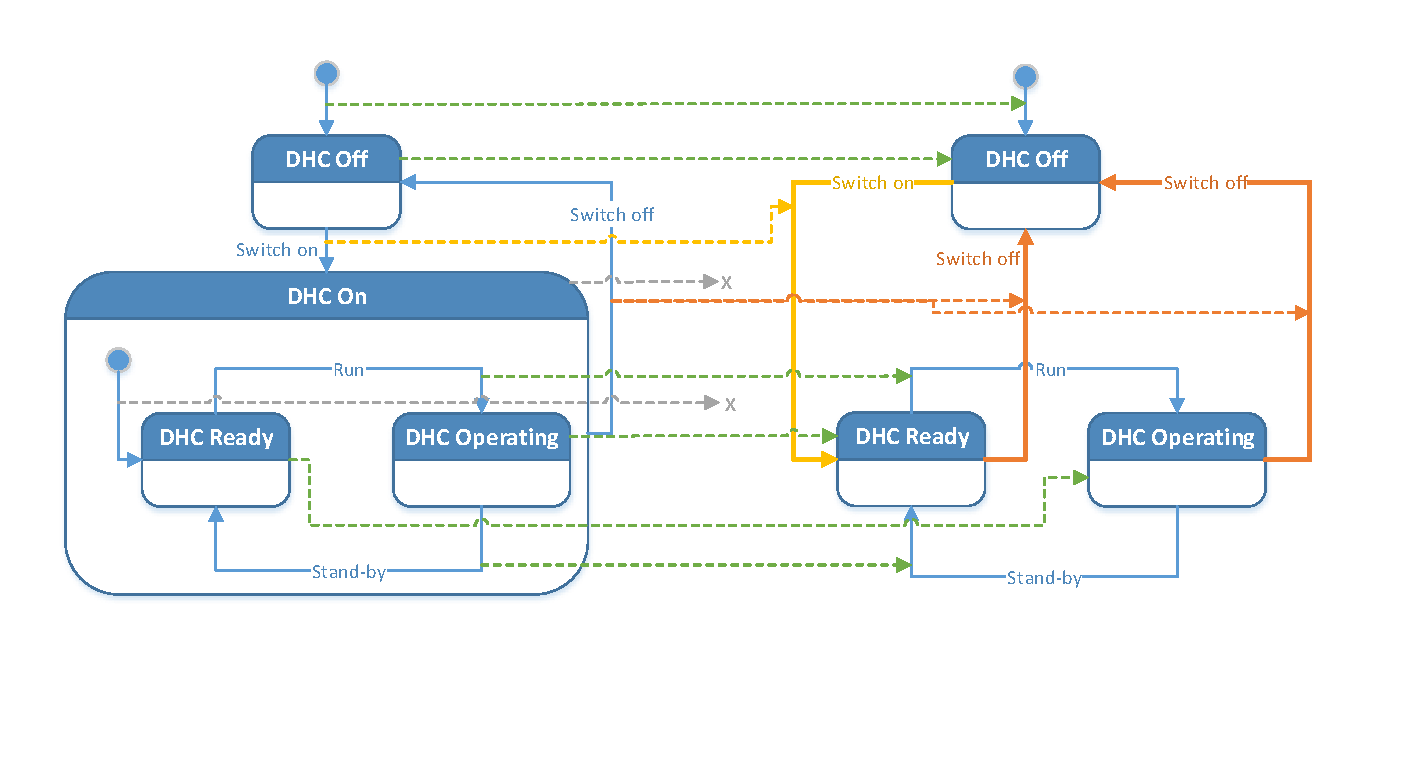
\includegraphics[scale=0.6, trim=0cm 1cm 0cm 1cm, clip=true]{Images/ScenarioBehavioralStateMachineTransformationOverview2.pdf} 
	\caption{Complex transformation scenario overview with \glspl{StateMachine} in \gls{ConcreteSyntax}}
	\label{figScenarioBehavioralStateMachineTransformationOverview2}
\end{figure}

While figure \ref{figScenarioBehavioralStateMachineTransformationOverview} highlights only the new transformation types, figure \ref{figScenarioBehavioralStateMachineTransformationOverview2} provides an overview of all required transformations for this example. Since the composite state has no equivalence, this results in a ``to zero" transformation. All other parts are transformed 1:1 on the \gls{MetaObjectFacility} \gls{Object} level, i.e. the state ``DHC Off". 
% transitions are not 1:1, the related \glspl{Association} change in these cases, too. An example is ``DHC Off", where in the complex-\gls{StateMachine} is one incoming and one outgoing transition, while in the simple-\gls{StateMachine} there are two incoming.

Following the same structure as in the simple scenario, in the next paragraphs the \glspl{MetaModel}, \glspl{ModelToModelTransformation} and the example \glspl{Model} are presented.

\begin{figure}[htb]
	\centering
	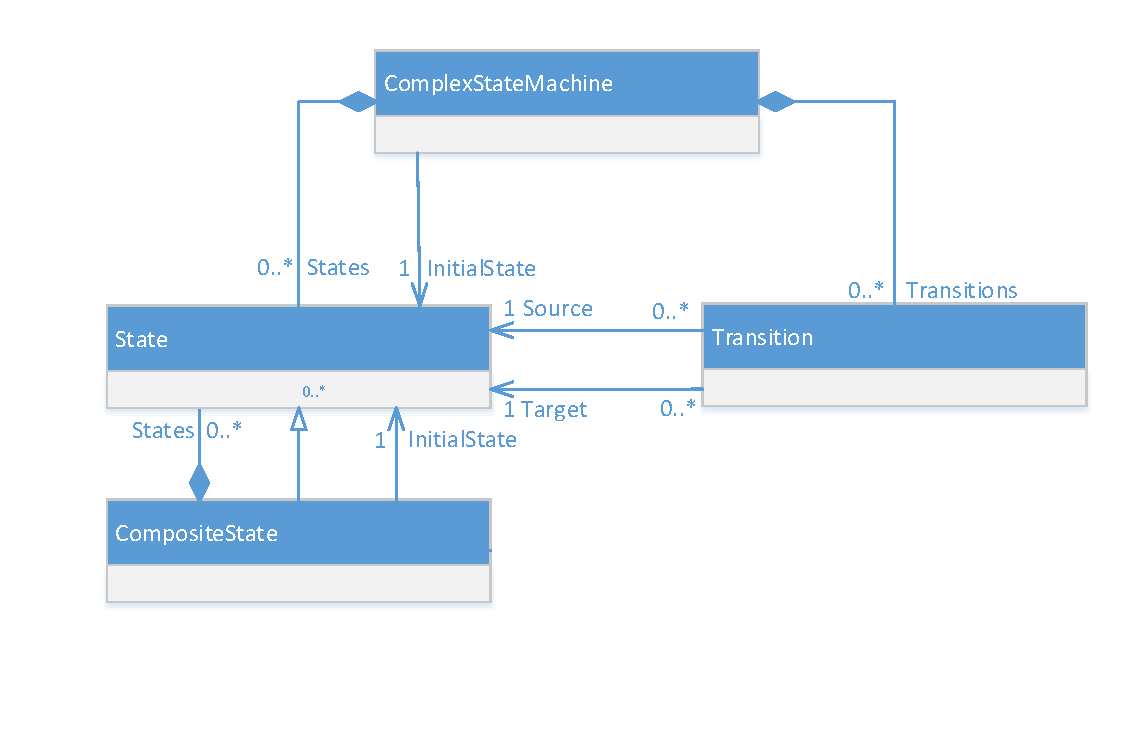
\includegraphics[scale=0.6, trim=0cm 1cm 0cm 1cm, clip=true]{Images/ScenarioBehavioralComplexStateMachine.pdf} 
	\caption{Complex State Machine - simplified \Gls{UnifiedModelingLanguage} \gls{StateMachine} \gls{MetaModel} with Composite States}
	\label{figScenarioBehavioralComplexStateMachine}
\end{figure}

The \gls{MetaModel} of the complex-\gls{StateMachine} is depicted in figure \ref{figScenarioBehavioralComplexStateMachine}. A ``ComplexStateMachine" consists of ``States" and ``Transitions" and defines an ``InitialState". A ``State" is connected by directed ``Transitions" to others and can also be a ``ComplexState". In this case it also contains ``States" and defines an ``InitialState".

\begin{figure}[htb]
	\centering
	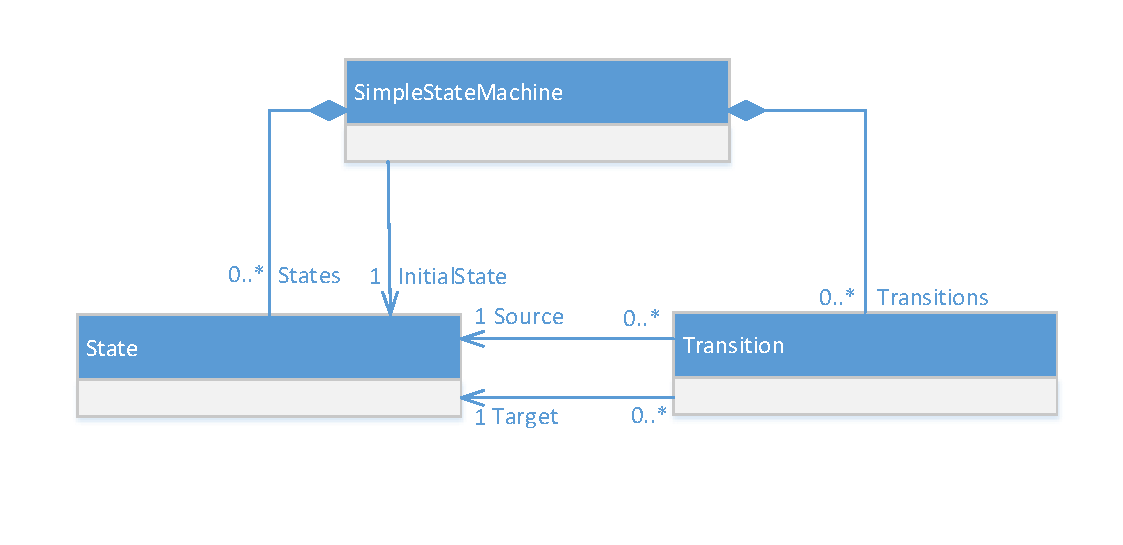
\includegraphics[scale=0.6, trim=0cm 1cm 0cm 1cm, clip=true]{Images/ScenarioBehavioralComplexSimpleStateMachine.pdf} 
	\caption{Simple State Machine - simplified \Gls{UnifiedModelingLanguage} \gls{StateMachine} \gls{MetaModel} without Composite States}
	\label{figScenarioBehavioralComplexSimpleStateMachine}
\end{figure}

The \gls{MetaModel} of the simple-\gls{StateMachine} is shown in figure \ref{figScenarioBehavioralComplexSimpleStateMachine}. It is identical to the complex type, except that the ``ComposisteState" is missing and that the name is ``SimpleStateMachine".

A \gls{ModelToModelTransformation} for those two \glspl{MetaModel} is defined in listing \ref{lstETLComplexExample}. There are multiple different transformations possible, depending on the approach. In this case, rules are defined for all \glspl{Class}, resulting in ``ComplexStateMachine To SimpleStateMachine", ``State To State", ``Transition To Transition". 

Since a transition is transformed differently depending on the context, there exists one rule for each, resulting in the additional rules ``TransitionPointingToComplexState To Transition" and ``TransitionFromComplexState To ManyTransitions". Another approach could be to handle all situations within one rule. Hence the used \gls{EpsilonTransformationLanguage} contains a concept called ``guards", which allows the definition of pre-conditions per rule, separate rules are defined to improve the readability. This solves the ``Context-dependent" challenge.

The ``One-to-one related" issue is solved in the rule ``TransitionPointingToComplexState To Transition", which covers all incoming ``Transitions" of a ``ComplexState". It defines a transformation from the ``InitialState" of the targeted ``ComplexState" towards the ``Target"-\gls{Property}. This change is also reflected in the mapping of the ``Name"-\gls{Property}. Another possible solution is to map the ``InitialState" of the ``ComplexState" by creating a further distinction of the ``State To State" rule. Since this does not remove the requirement for the ``TransitionPointingToComplexState To Transition" rule, this solution would result in a more complicated transformation.

The ``One-to-many" challenge is handled within the rule ``TransitionFromComplexState To ManyTransitions", which handles all outgoing ``Transitions" of a ``ComplexState". Here, the ``States" of the ``ComplexState" are enumerated and for each a new ``Transition" is created. The ``Source" is the current ``State", while the ``Target" is equivalent to the one of the handled ``Transition". This relationship is reflected in the ``Name" of the new ``Transition". As well as in the previous case, this can also be solved by a dedicated ``State To State" rule, which would result in a less comprehensible transformation.

\begin{lstlisting}[language=ETL,caption={Complex State Machine to Simple State Machine \gls{ModelToModelTransformation} in \gls{ConcreteSyntax} of \Gls{EpsilonTransformationLanguage}},label={lstETLComplexExample}]
rule ComplexStateMachineToSimpleStateMachine
	transform complexStateMachine : Source!ComplexStateMachine
	to simpleStateMachine : Target!SimpleStateMachine {
	
	simpleStateMachine.Name = complexStateMachine.Name;
	simpleStateMachine.InitialState = 
								complexStateMachine.InitialState.equivalent();
}

rule StateToState
	transform sourceState : Source!State
	to targetState : Target!State {
	
	targetState.Name = sourceState.Name;	
	targetState.SimpleStateMachine = 
								sourceState.ComplexStateMachine.equivalent();
}

rule TransitionToTransition
	transform sourceTransition : Source!Transition
	to targetTransition : Target!Transition {
	guard : 	not sourceTransition.Target.isTypeOf(Source!CompositeState)
		    and not sourceTransition.Source.isTypeOf(Source!CompositeState) 
	
	targetTransition.SimpleStateMachine = 
								sourceTransition.ComplexStateMachine.equivalent();
	targetTransition.Name = sourceTransition.Name;
	targetTransition.Source = sourceTransition.Source.equivalent();	
	targetTransition.Target = sourceTransition.Target.equivalent();
}

rule TransitionPointingToComplexStateToTransition
	transform sourceTransition : Source!Transition
	to targetTransition : Target!Transition { 
	guard : sourceTransition.Target.isTypeOf(Source!CompositeState)
			and not sourceTransition.Source.isTypeOf(Source!CompositeState)
	
	targetTransition.Name = sourceTransition.Source.Name + " -> " + 
							sourceTransition.Target.InitialState.Name;
	targetTransition.Source = sourceTransition.Source.equivalent();
	targetTransition.Target = sourceTransition.Target.InitialState.equivalent();

	targetTransition.SimpleStateMachine = 
								sourceTransition.ComplexStateMachine.equivalent();
}

rule TransitionFromComplexStateToManyTransitions
	transform sourceTransition : Source!Transition
	to targetTransitions : Sequence(Target!Transition) {
	guard : sourceTransition.Source.isTypeOf(Source!CompositeState)
			and not sourceTransition.Target.isTypeOf(Source!CompositeState)

	for(sourceState in sourceTransition.Source.States) {
		var targetTransition = new Target!Transition;
		targetTransitions.add(targetTransition);
		
		targetTransition.Name = sourceState.Name + " -> " + 
								sourceTransition.Target.Name;
		targetTransition.Source = sourceState.equivalent();
		targetTransition.Target = sourceTransition.Target.equivalent();
		
		targetTransition.SimpleStateMachine = 
								sourceTransition.ComplexStateMachine.equivalent();
	}
}
\end{lstlisting}

The described \gls{ModelToModelTransformation} results in the following changes of a \gls{Model}, which is the example used to guide the \gls{TransformationGenerator}. Those are in the \gls{AbstractSyntax}, to be able to present all involved \gls{MetaObjectFacility} elements as they are handled by the \gls{TransformationGenerator}.

\begin{figure}[htb]
	\centering
	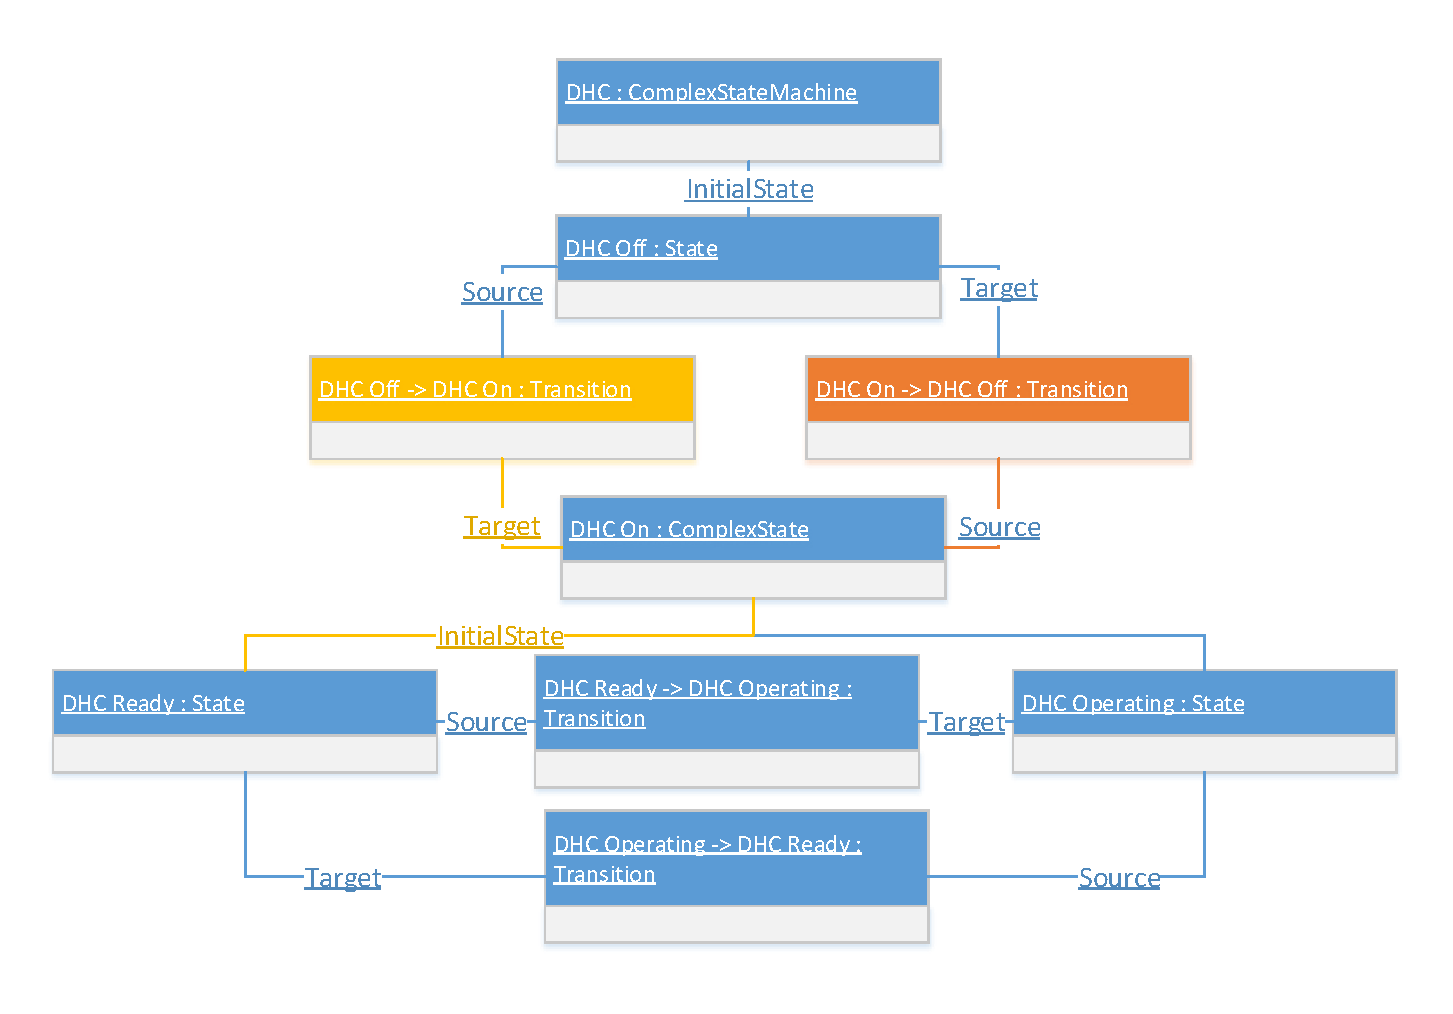
\includegraphics[scale=0.6, trim=0cm 1cm 0cm 1cm, clip=true]{Images/ScenarioBehavioralComplexStateMachineModel1.pdf} 
	\caption{Complex State Machine example \gls{Model} in \gls{AbstractSyntax} (without the associations from the ComplexStateMachine to all other \glspl{Object})}
	\label{figScenarioBehavioralComplexStateMachineModel1}
\end{figure}

Figure \ref{figScenarioBehavioralComplexStateMachineModel1} shows the input \gls{Model} M$_a$ and figure \ref{figScenarioBehavioralComplexSimpleStateMachineModel1} the output \gls{Model} M$_b$, based on the already introduced example. The highlighted parts correspond to the previously defined challenges in figure \ref{figScenarioBehavioralStateMachineTransformationOverview}.

The ``TransitionPointingToComplexState To Transition"-rule changes the ``DHC Off  $\rightarrow$  DHC On"-"Transition" into ``DHC Off  $\rightarrow$  DHC Ready". ``TransitionFromComplexState To ManyTransitions" replaces the ``DHC On  $\rightarrow$  DHC Off"-"Transition" with the two inner ``States" of the ``ComplexState".

\begin{figure}[htb]
	\centering
	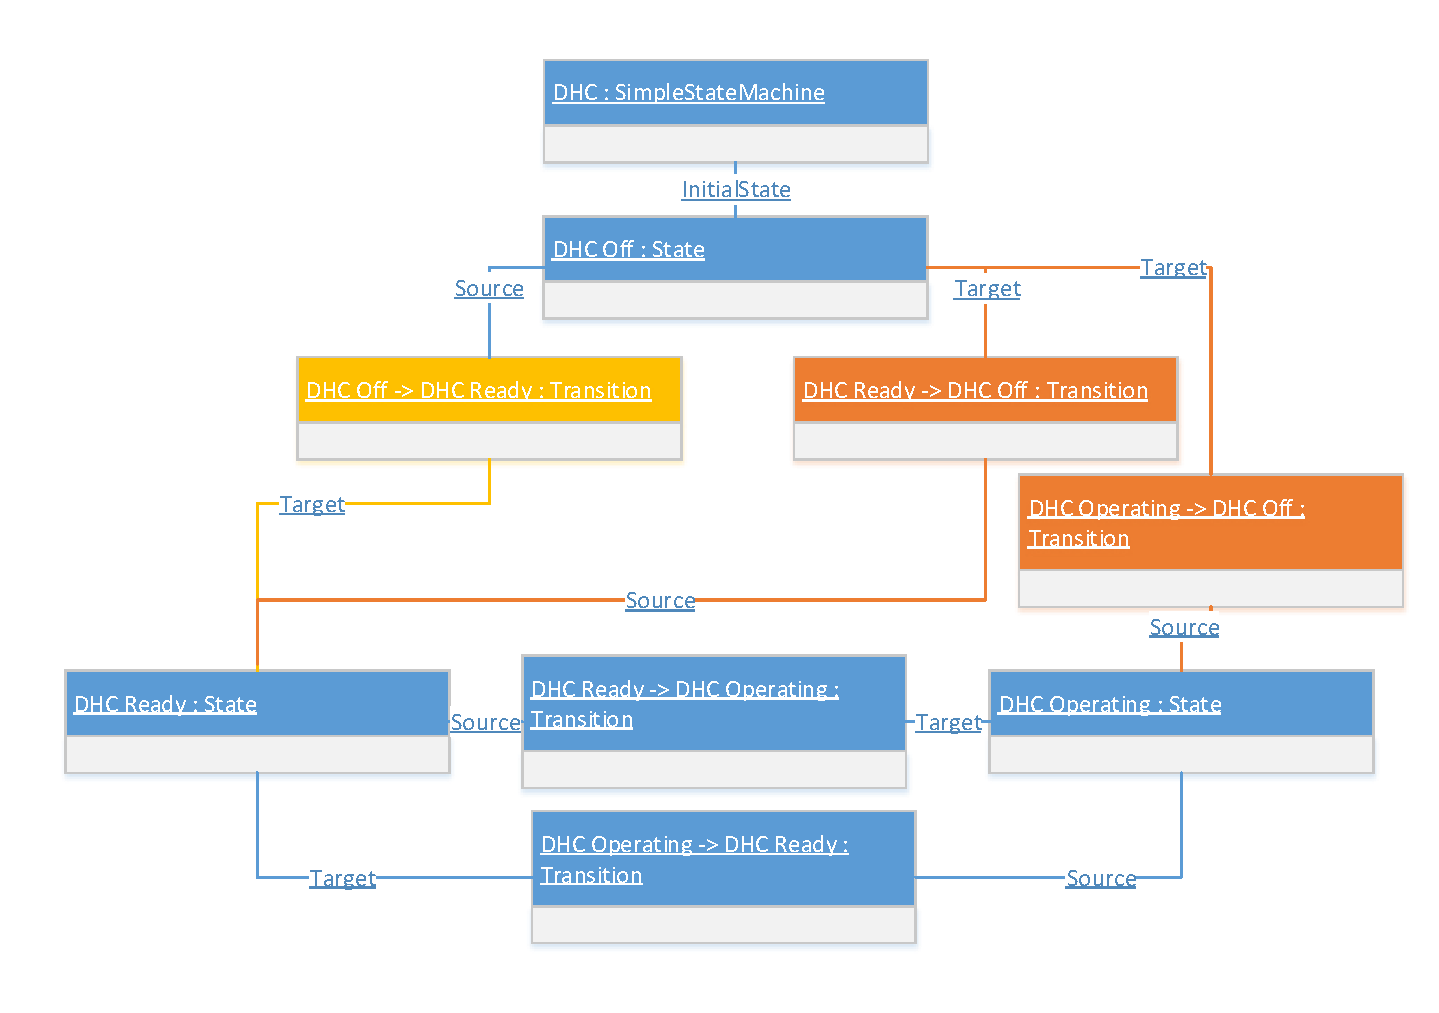
\includegraphics[scale=0.6, trim=0cm 1cm 0cm 1cm, clip=true]{Images/ScenarioBehavioralComplexSimpleStateMachineModel1.pdf} 
	\caption{Simple State Machine example \gls{Model} in \gls{AbstractSyntax} (without the associations from the SimpleStateMachine to all other \glspl{Object})}
	\label{figScenarioBehavioralComplexSimpleStateMachineModel1}
\end{figure}



